\section{Experiments and Results}

% \uselengthunit{in}\printlength{\textwidth} = 4.8041 in
% \uselengthunit{mm}\printlength{\textwidth} = 121.99854 mm

To allow for a direct comparison with state-of-the-art lesion segmentation
methods, we evaluated our method on the FLAIR, T1-, and T2-weighted MRIs of the
20 publicly available labeled cases from the MS lesion segmentation challenge
2008 \cite{styner20083d}, which we downsampled from the original isotropic voxel
size of \SI{0.5}{\cubic\milli\metre} to an isotropic voxel size of
\SI{1.0}{\cubic\milli\metre}. In addition, we evaluated our method on an
in-house data set from an MS clinical trial of 500 subjects split equally into
training and test sets. The images were acquired from 45 different scanning
sites. For each subject, the data set contains T2- and PD-weighted MRIs with a
voxel size of \SI{0.937x0.937x3.000}{\milli\metre}. The main preprocessing steps
included rigid intra-subject registration, brain extraction, intensity
normalization, and background cropping.
%  To compute a lesion distribution map, we affinely registered the training
% subjects of our in-house data set to MNI space and calculated the average
% lesion mask. We used the square root of the average lesion mask as a prior to
% counterbalance large differences in lesion probability between regions and
% added the lesion prior as an additional input channel to both data sets.
%  We used a CEN with 32 filters and filter sizes of \num{9x9x9} and \num{9x9x5}
% voxels for the challenge and in-house data sets, respectively. Training on a
% single GeForce GTX 780 graphics card took between 24 and 32 hours per model.
% However, once the network is trained, segmentation of new images can be
% performed in less than one second.

We used a CEN with 32 filters and filter sizes of \num{9x9x9} and \num{9x9x5}
voxels for the challenge and in-house data sets, respectively. Training on a
single GeForce GTX 780 graphics card took between 6 and 32 hours per model
depending on the training set size. However, once the network is trained,
segmentation of trimodal 3D volumes with a resolution of, e.g.,
\num{159x201x155} voxels can be performed in less than one second. As a
rough\footnote{Ciresan et al. used a more complex network that is composed of 11
layers. However, their network was trained on much smaller images, which roughly
compensates for the increased complexity.} comparison, Ciresan et al.
\cite{Ciresan2012} reported that their patch-based method required 10 to 30
minutes to segment a single 2D image with a resolution of \num{512x512} voxels
using four graphics cards, which demonstrates the large speed-ups gained by
processing entire volumes.

\begin{figure}[tb]
\centering
\small
%\def\MRIwidth{0.159\textwidth}
\def\MRIwidth{0.15\textwidth}

\begin{tikzpicture} 
\tikzstyle{leftlabel}=[rotate=90, align=center,overlay,above]

\matrix [matrix of nodes, nodes={anchor=center, inner sep=1pt}] {
        &[4pt] FLAIR & T1w & T2w & Ground truth & Our method \\[4pt]
\node[leftlabel] {CHB\,07\\(DSC\,=\,\SI{60.58}{\percent})}; &
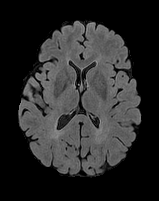
\includegraphics[width=\MRIwidth]{figures/CHB07-FLAIR-s88} &
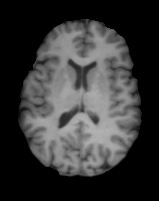
\includegraphics[width=\MRIwidth]{figures/CHB07-T1w-s88} &
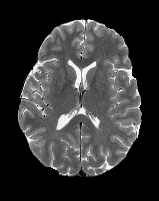
\includegraphics[width=\MRIwidth]{figures/CHB07-T2w-s88} &
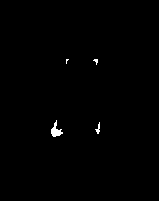
\includegraphics[width=\MRIwidth]{figures/CHB07-gold-s88} &
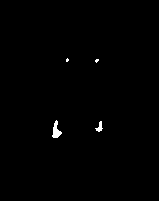
\includegraphics[width=\MRIwidth]{figures/CHB07-pred-s88} \\
\node[leftlabel] {CHB\,04\\(DSC\,=\,\SI{61.37}{\percent})}; &
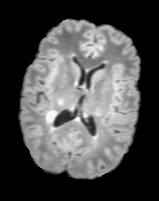
\includegraphics[width=\MRIwidth]{figures/CHB04-FLAIR-s85} &
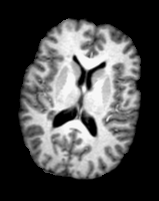
\includegraphics[width=\MRIwidth]{figures/CHB04-T1w-s85} &
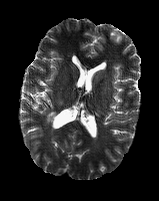
\includegraphics[width=\MRIwidth]{figures/CHB04-T2w-s85} &
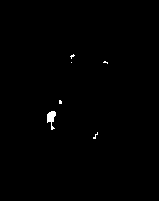
\includegraphics[width=\MRIwidth]{figures/CHB04-gold-s85} &

\includegraphics[width=\MRIwidth]{figures/CHB04-pred-s85} \\
\node[leftlabel] {UNC\,09\\(DSC\,=\,\SI{9.01}{\percent})}; &
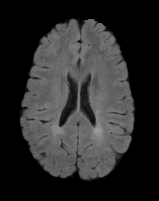
\includegraphics[width=\MRIwidth]{figures/UNC09-FLAIR-s89} &
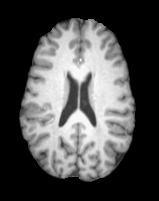
\includegraphics[width=\MRIwidth]{figures/UNC09-T1w-s89} &
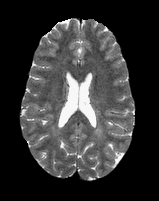
\includegraphics[width=\MRIwidth]{figures/UNC09-T2w-s89} &

\includegraphics[width=\MRIwidth]{figures/UNC09-gold-s89} &

\includegraphics[width=\MRIwidth]{figures/UNC09-pred-s89} \\
};
\end{tikzpicture}

\caption{Example segmentations of our method for three different subjects from
the challenge data set. Our method performed well and consistently despite the
large contrast differences seen between the first two rows. In the third row,
our method also segmented lesions that have similar contrast, but these regions
had not been identified as lesions by the manual rater, which highlights the
difficulty in distinguishing focal lesions from diffuse damage, even for
experts.}

\label{fig:segmentation}
\end{figure}

We evaluated our method on the challenge data set using 5-fold
cross-valida\-tion and calculated the true positive rate (TPR), positive
predictive value (PPV), and Dice similarity coefficient (DSC) between the
predicted segmentations and the resampled ground truth.
Figure~\ref{fig:segmentation} shows a comparison of three subjects from the
challenge data set. The first two rows show the FLAIR, T1w, T2w, ground truth
segmentations, and predicted segmentations of two subjects with a DSC of
\SI{60.58}{\percent} and \SI{61.37}{\percent}. Despite the large contrast
differences between the two subjects, our method performed well and
consistently, which indicates that our model was able to learn features that are
robust to a large range of intensity variations. The last row shows a subject
with a DSC of \SI{9.01}{\percent}, one of the lowest DSC scores from the data
set. Our method segmented lesions that have similar contrast to the other two
subjects, but these regions were not classified as lesions by the manual rater.
This highlights the difficulty of manual lesion segmentation, as the difference
between diffuse white matter pathology and focal lesions is often indistinct. A
quantitative comparison of our method with other state-of-the-art methods is
summarized in Table~\ref{tab:state}. Our method outperforms the winning method
(Souplet et al. \cite{souplet2008}) of the MS lesion segmentation challenge 2008
and the currently best unsupervised method reported on that data set (Weiss et
al. \cite{weiss2013}) in terms of mean TPR and PPV. Our method performs
comparably to a current method (Geremia et al. \cite{geremia2010}) that uses a
carefully designed set of features specifically designed for lesion
segmentation, despite our method having learned its features solely from a
relatively small training set.

\begin{table}[tb]
\def\tabspace{12pt}

\caption{Comparison of our method with state-of-the-art lesion segmentation
methods in terms of mean TPR, PPV, and DSC. Our method performs comparably to
the best methods reported on the MS lesion segmentation challenge data set.}

\label{tab:state}
\centering
\begin{tabular}{l%
@{\hspace{\tabspace}}S[table-format=2.2]
@{\hspace{\tabspace}}S[table-format=2.2]
@{\hspace{\tabspace}}S[table-format=2.2]
}
\toprule
Method & {TPR} & {PPV} & {DSC} \\ 
\midrule
Souplet et al. \cite{souplet2008} & 20.65 & 30.00 & {---} \\ 
Weiss et al. \cite{weiss2013} & 33.00 & 36.85 & 29.05 \\ 
Geremia et al. \cite{geremia2010} & 39.85 & 40.35 & {---}  \\
Our method & 39.71 & 41.38 & 35.52 \\
\bottomrule
\end{tabular}
\end{table}

To evaluate the impact of the training set size on the segmentation performance,
we trained our model on our in-house data set with a varying number of training
samples and calculated the mean DSC on the training and test sets as illustrated
in Fig.~\ref{fig:bioms}. For small training sets, there is a large difference
between the DSCs on the training and test sets, which indicates that the
training set is too small to learn a representative set of features. At around
100 samples, the model becomes stable in terms of test performance and the small
difference between training and test DSCs, indicating that overfitting of the
training data is no longer occurring. With 100 training subjects, our method
achieves a mean DSC on the test set of \SI{57.38}{\percent}, which shows that
the segmentation accuracy can be greatly improved compared to the results on the
challenge data set, when a representative training set is available.

\begin{figure}[tb]
\centering
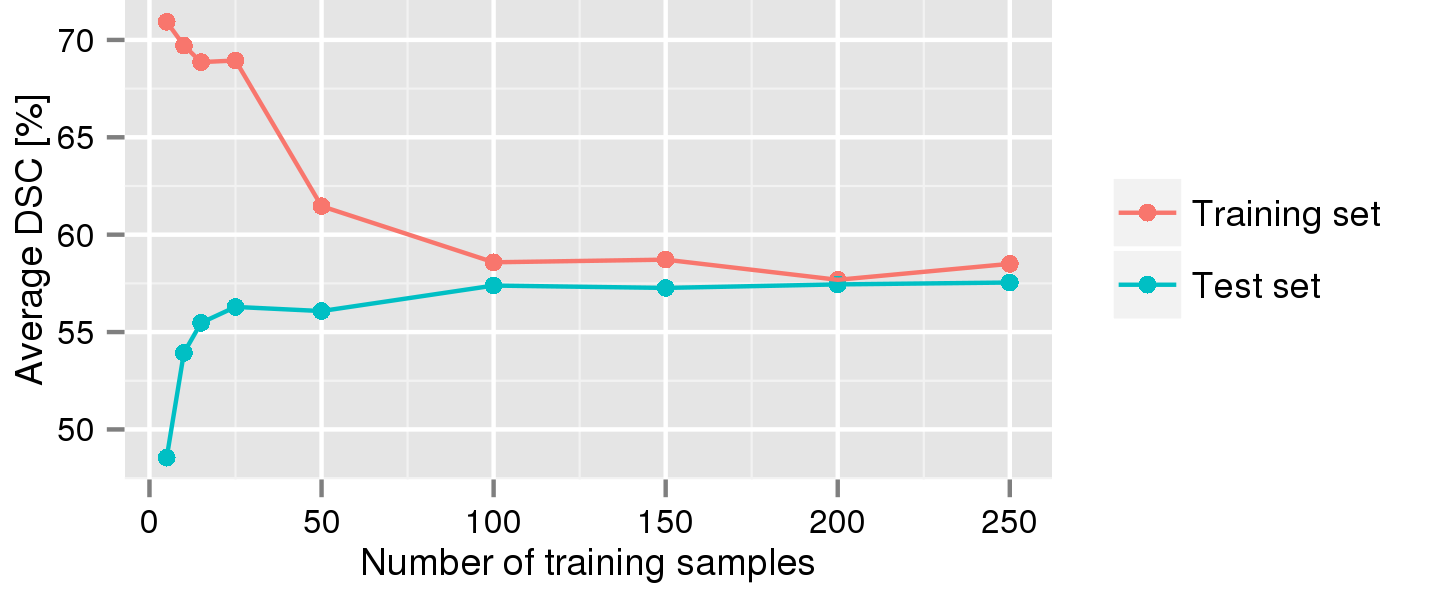
\includegraphics[width=0.78\textwidth]{figures/train_count}

\caption{Comparison of DSC scores calculated on the training and test sets for
varying numbers of training samples. At around 100 samples, the model becomes
stable in terms of test performance and the small difference between training
and test DSCs, indicating that overfitting of the training data no longer
occurs.}
\label{fig:bioms}
\end{figure}

% We have evaluated our method on two data sets. To allow for a direct comparison
% to other state of the art lesion segmentation methods, we have evaluated our
% method on the 20 labeled cases from the MICCAI lesion segmentation challenge
% \cite{styner20083d}. FLAIR, T1, T2, The preprocessing pipeline includes, global
% contrast normalization, resampling of the images to a voxel size of
% \SI{1}{\cubic\milli\metre}, intra-subject registration to the FLAIR images,
% brain extraction using BET, and cropping to a revolution of \num{159x201x155} voxels.
% To account for the spatial location of lesion, we have added a lesion prior as a
% forth channel, which captures the average lesion distribution of 500 subjects
% from an MS clinical trial. Training was performed using 5-fold cross-validation
% with the following parameters: 32 filters with a filter size of \num{9x9x9} and
% a sensitivity ratio of $0.02$. The model was trained for 4000 epochs. Training
% of a single split took approximately 36 hours on a single GeForce GTX 760
% graphics card. Once the model is trained, segmentation of a single image can be
% performed in less than one second.

% To evaluate the impact of the training set size on the learned model, we have
% also evaluated our method on a data set of 500 T2 and PD weighted images from an
% MS clinical trials with a voxel size of \SI{1x1x3}{\milli\metre}. The
% pre-processing pipeline includes global contrast normalization, intra-subject
% registration, brain extraction, and cropping to a resolution of
% \num{159x207x53}.
% To evaluate the impact of the training set size on the segmentation performance,
% we have evaluated our model on different subsets of a data set from an MS clinical
% trail. With data set contained T2w and PDw images from 500 subjects at a single
% time point.

% We have divided the data set into a training and test set containing
% 250 images each. We have then trained our model on a varying number of image
% from the training set and evaluated the segmentation performance on the
% selected training samples and all images of the test set. The result of this
% test is illustrated in Table~\ref{tab:bioms}. For very small number of training
% samples, our model achieves a DSC of 71 in the training set and 49 in the test
% set. The large difference between the results on the training and test set
% indicates that the training sample size is not sufficient to prevent
% overfitting. As we increase the number of training samples, the difference
% between the results on the training and test set decreases. At 150 samples, the
% performance on the training set is almost as good as on the test set, which
% indicates that our model is not overfitting. We also do not see an improvement
% thereafter. For this study, if have trained a relatively simple model with only
% 2 layers and 32 filters per layer. We expect that models with more layers and
% filters are more prone to overfitting for smaller training set sizes, but might
% keep improving beyond 150 samples.

% \paragraph{Training Pipeline}
% \begin{itemize}
% \item Downsample training images and training segmentations from
% \SI{0.5x0.5x0.5}{\milli\meter} to \SI{1x1x1}{\milli\meter} voxel resolution.
% \item Perform brain extraction
% \item Crop to smallest ROI
% \item Pad all images to standard size
% \item[$\Rightarrow$] Calculate combined cropping parameters
% \item Perform training of the NN on the downsampled training set
% \item Calculate probability maps for the entire downsampled training set
% \item Upsample the probability maps to the native resolution
% \item Crop lesion masks in native resolution to fit the same ROI as the
% upsampled probability masks
% \item Choose the threshold that maximizes the DSC in the training set 
% \end{itemize}

% \paragraph{Experiments to come}
% 
% \begin{itemize}
% 
% \item \emph{Optional}\quad Evaluation on BioMS using stride-1 convolutions and
% new pre-processing pipeline with and without lesion prior, with individual and
% shared bias terms. Metrics: TPR, PPV, DSC, correlations with lesion load and
% clinical scores.
% 
% \end{itemize}


% \begin{table}
% \caption{Segmentation results measured using the Dice Similarity Coefficient.
% Two layer auto-encoder, stride size of \num{2x2x1}, 32 filters, sensitivity
% ratio 0.05. Threshold finding methods: a) using a global threshold that
% optimizes the average DSC of the entire data set, b) using the optimal
% thresholds for each sample, and c) using predicted thresholds for each sample.}
% \label{tab:segmentation}
% \centering
% \def\tabspace{10pt}
% \sisetup{
%   round-precision = 3,
% }%
% % \small
% \begin{tabular}{@{}l%
% @{\hspace{\tabspace}}S[table-format=1.3]%
% @{\hspace{\tabspace}}S[table-format=1.3]
% @{\hspace{\tabspace}}S[table-format=1.3]
% @{\hspace{\tabspace}}S[table-format=1.3]
% @{\hspace{\tabspace}}S[table-format=1.3]
% @{\hspace{\tabspace}}S[table-format=1.3]
% @{}}
% \toprule
% Method & \multicolumn{6}{c}{DSC per Lesion Load Category} \\
% \addlinespace
%  & {0.0--4.0} & {4.0--7.8} & {7.8--14.7} & {14.7--28.5} & {$>28.5$} &
% {Average} \\
% \midrule
% Global threshold &  0.297805 & 0.545574 & 0.60051 & 0.650483 & 0.679614 &
%  0.543181 \\
% Optimal thresholds & 0.351185 & 0.568412 & 0.618115 & 0.667473 & 0.727397 &
% 0.572716 \\
% Predicted thresholds & 0.337834 & 0.550028 & 0.587458 & 0.653475 &
% 0.716976 & 0.555662 \\
% \bottomrule
% \end{tabular}
% \end{table}
% 
% \begin{table}
% \caption{Correlations with biomarkers is comparable to the expert
% segmentations. Threshold methods are: global threshold (LLG), optimal threshold
% (LLO), and predicted threshold (LLP).}
% \label{tab:cross}
% \centering
% \def\tabspace{14pt}
% \begin{tabular}{c%
% @{\hspace{\tabspace}}S[table-format=1.4]%
% @{\hspace{\tabspace}}S[table-format=2.6]%
% @{\hspace{\tabspace}}S[table-format=2.6]%
% @{\hspace{\tabspace}}S[table-format=2.6]%
% @{\hspace{\tabspace}}S[table-format=1.5]%
% @{\hspace{\tabspace}}S[table-format=1.6]%
% }
% \toprule
%      & {T25W} & {9-HPT} & {PASAT} & {MSFC} & {EDSS} & {T2LL} \\
% \midrule
% LLG & 0.0889204058874592 & -0.299046682079096*** & -0.35652944988915*** & -0.414587036427664*** & 0.111910491023784* & 0.867904019287295*** \\
% LLO & 0.0955077933828887* & -0.29002627967845*** & -0.36828512897955*** & -0.41898534832637*** & 0.116889743878327* & 0.988979555746338*** \\
% LLP & 0.0896915607291051 & -0.300773510817976*** & -0.342386015914701*** & -0.411524441008343*** & 0.134054634214833** & 0.869216107742852*** \\
% \addlinespace
% T2LL & 0.0830609699877066 & -0.288809520550953*** & -0.370891003440786*** &
% -0.415459123322053*** & 0.121219714387235* & {---} \\
% \bottomrule
% \end{tabular}
% \end{table}

